\documentclass[11pt, a4paper]{article}
\usepackage[T1]{fontenc}
\usepackage{lmodern}
\usepackage[margin=1in]{geometry}
\usepackage{amsmath, amssymb}
\usepackage{tikz}
\usepackage{tcolorbox}
\usepackage{xcolor}

\definecolor{primary}{HTML}{2B3A42}
\definecolor{accent}{HTML}{3F5765}
\definecolor{highlight}{HTML}{EFEFEF}
\definecolor{profbg}{HTML}{F4F8FA}
\definecolor{profframe}{HTML}{4A7C82}

\tcbset{
    profbox/.style={
        colback=profbg,
        colframe=profframe,
        fonttitle=\bfseries,
        arc=2pt,
        boxrule=1pt,
        left=6pt, right=6pt, top=6pt, bottom=6pt
    }
}

\title{\textbf{Descriptive Statistics}\\
\large Mathematics for Computing}
\author{Augustin Thomas}
\date{September 1, 2026}

\begin{document}
\maketitle
\vspace{-1.5cm}

\section{Introduction to Univariate Data and Order Statistics}
Univariate data involves the observation of a single random variable $X$. A sample of size $n$, denoted as $x_1, x_2, \dots, x_n$, is drawn from an unknown underlying population distribution. To analyze empirical properties without parametric assumptions, we rely on \textbf{order statistics}. Sorting the sample in ascending order yields the sequence $x_{(1)} \le x_{(2)} \le \dots \le x_{(n)}$, where $x_{(1)}$ is the sample minimum and $x_{(n)}$ is the sample maximum.

\begin{tcolorbox}[profbox, title=Imagine: The Roll Call]
Imagine an unorganized crowd of students in a gymnasium. This is your raw sample. Order statistics is the act of forcing them to stand in a single straight line sorted exactly by height. Suddenly, the shortest student ($x_{(1)}$) and the tallest ($x_{(n)}$) are instantly visible at the extremes. By simply organizing the data geographically, non-parametric structures reveal themselves without assuming the crowd follows a "normal" bell-curve of heights.
\end{tcolorbox}

\vspace{0.3cm}
\noindent\fbox{%
    \parbox{0.95\textwidth}{%
        \textbf{Working Example: Edge Device Inference Time}\\
        Consider a sample representing the execution time (in milliseconds) of an AI model running on an edge device.\\
        \textbf{Raw data ($n=9$):} 14, 18, 12, 45, 16, 14, 22, 19, 15\\
        \textbf{Order Statistics:} 12, 14, 14, 15, 16, 18, 19, 22, 45
    }%
}
\vspace{0.3cm}

\section{Measures of Central Tendency}
Central tendency is a single summary value that describes the center point or typical position of a data set.

\begin{itemize}
    \item \textbf{Sample Mean ($\bar{x}$):} The arithmetic average. By the Law of Large Numbers, it provides a consistent estimator for the population mean $\mu$. 
    \[ \bar{x} = \frac{1}{n} \sum_{i=1}^{n} x_i \]
    
    \item \textbf{Sample Median ($\tilde{x}$):} The 50th percentile. It is highly robust to outliers compared to the mean.
    \[ 
    \tilde{x} = 
    \begin{cases} 
    x_{((n+1)/2)} & \text{if } n \text{ is odd} \\
    \frac{1}{2} \left( x_{(n/2)} + x_{(n/2 + 1)} \right) & \text{if } n \text{ is even} 
    \end{cases} 
    \]
    
    \item \textbf{Mode:} The most frequent value, representing the peak(s) of the estimated density function.
\end{itemize}

\begin{tcolorbox}[profbox, title=Imagine: The Seesaw vs. The Middle Child]
\textbf{The Mean is a seesaw.} Imagine: a rigid plank (number line) with weights placed at each data point. The mean is the exact fulcrum point where the seesaw perfectly balances. If you move one weight extremely far to the right (an outlier like 45ms), you must drag the fulcrum far to the right to prevent the seesaw from tipping. \\
\textbf{The Median is the middle child.} You line up 9 people by wealth. The 5th person is the median. If the 9th person is suddenly replaced by Jeff Bezos, the 5th person's wealth doesn't change at all. The median cares about \textit{rank}, not \textit{magnitude}, making it bulletproof against extreme anomalies.
\end{tcolorbox}

\section{Measures of Dispersion}
Dispersion quantifies the spread of the data. Accurately modeling variance is critical for computing the mean square error (MSE) and confidence intervals during parameter estimation.

\begin{itemize}
    \item \textbf{Sample Variance ($s^2$):} The average squared deviation from the mean. To ensure the estimator is unbiased ($E[s^2] = \sigma^2$), we apply Bessel's correction ($n-1$).
    \[ s^2 = \frac{1}{n-1} \sum_{i=1}^{n} (x_i - \bar{x})^2 \]
    
    \item \textbf{Sample Standard Deviation ($s$):} The square root of the variance ($s = \sqrt{s^2}$).
    
    \item \textbf{Range:} The absolute spread given by $x_{(n)} - x_{(1)}$.
\end{itemize}

\begin{tcolorbox}[profbox, title=Imagine: The Archer's Target]
Think of the Mean as the bullseye on an archery target. The \textbf{Standard Deviation} is the radius of a circle around the bullseye that captures the majority of your arrows. A small standard deviation means you are a highly consistent archer (tight grouping). A large standard deviation means your arrows are scattered wildly across the target. \\
\textit{Why square the distances for Variance?} Squaring acts like a statistical magnifying glass—it brutally penalizes arrows that land extremely far away, forcing our models to pay strict attention to large errors (which is why MSE is foundational in machine learning).
\end{tcolorbox}

\section{Quartiles, IQR, and Outlier Detection}
Quartiles segment the order statistics into four equal probability mass regions.

\begin{itemize}
    \item \textbf{First Quartile ($Q_1$):} Median of the lower half of the data (25th percentile). 
    \item \textbf{Third Quartile ($Q_3$):} Median of the upper half of the data (75th percentile).
    \item \textbf{Interquartile Range (IQR):} Measures the core spread of the data, $IQR = Q_3 - Q_1$.
\end{itemize}

\subsection*{Tukey's Fences for Outliers}
Extreme values can heavily penalize parametric model estimators. Tukey's rule defines an outlier $x_i$ if it falls outside the interval:
\[ \left[ Q_1 - 1.5 \times IQR, \quad Q_3 + 1.5 \times IQR \right] \]

\begin{tcolorbox}[profbox, title=Imagine: The Statistical Sandwich]
If your dataset is a sandwich, $Q_1$ and $Q_3$ are the slices of bread. The \textbf{IQR} is the meat inside—it holds the dense, central 50\% of your data's nutritional value. When we look for outliers using Tukey's Fences, we are simply looking for crumbs that fell way outside the plate. If a data point lands more than 1.5 times the width of the sandwich away from the bread, we flag it as an outlier (like our 45ms inference time).
\end{tcolorbox}

\section{Visualizing Univariate Data: The Box Plot}
A box plot maps the non-parametric five-number summary: (Min, $Q_1$, Median, $Q_3$, Max), visualizing spread and skewness simultaneously.

\vspace{0.5cm}
\begin{center}
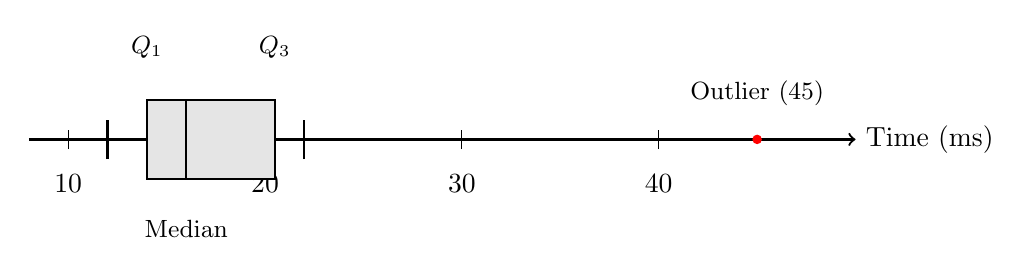
\begin{tikzpicture}[scale=0.25]
    % X-Axis
    \draw[->, thick] (8,0) -- (50,0) node[right] {Time (ms)};
    \foreach \x in {10, 20, 30, 40} {
        \draw (\x, -0.5) -- (\x, 0.5);
        \node[below=0.2cm] at (\x, -0.5) {\x};
    }
    
    % Box (Q1 to Q3)
    \filldraw[fill=gray!20, draw=black, thick] (14, -2) rectangle (20.5, 2);
    
    % Median
    \draw[thick, draw=black] (16, -2) -- (16, 2);
    
    % Whiskers
    \draw[thick, draw=black] (12, 0) -- (14, 0);
    \draw[thick, draw=black] (20.5, 0) -- (22, 0);
    
    % Whisker ends
    \draw[thick, draw=black] (12, -1) -- (12, 1);
    \draw[thick, draw=black] (22, -1) -- (22, 1);
    
    % Outlier
    \filldraw[red] (45,0) circle (6pt);
    \node[above=0.3cm] at (45,0) {\small Outlier (45)};
    
    % Labels
    \node[below=0.4cm] at (16, -2) {\small Median};
    \node[above=0.4cm] at (14, 2) {\small $Q_1$};
    \node[above=0.4cm] at (20.5, 2) {\small $Q_3$};
\end{tikzpicture}
\end{center}
\vspace{0.2cm}

\begin{tcolorbox}[profbox, title=Imagine: The City Map]
View the box plot as a top-down drone shot of a city's population density. The central gray box is the downtown metropolitan core (where 50\% of the population lives packed together). The median line is Main Street. The whiskers are the sprawling suburbs. That red dot out at 45? That's a solitary cabin in the remote wilderness.
\end{tcolorbox}

\section{Shape Characteristics: Skewness and Kurtosis}
Beyond central tendency and variance, higher-order standardized moments characterize the empirical distribution's overall shape.

\subsection*{Skewness ($g_1$)}
Skewness quantifies the asymmetry of the probability distribution. Based on the 3rd standardized moment:
\[ g_1 = \frac{\frac{1}{n} \sum_{i=1}^{n} (x_i - \bar{x})^3}{\left( \frac{1}{n} \sum_{i=1}^{n} (x_i - \bar{x})^2 \right)^{3/2}} \]

\vspace{0.2cm}
\begin{center}
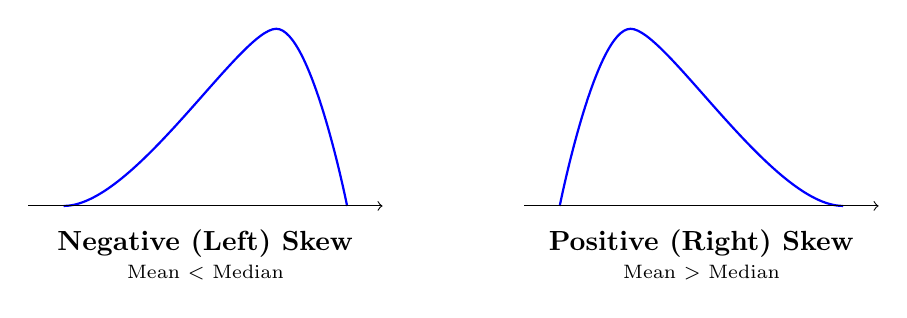
\begin{tikzpicture}[scale=0.9]
    % Negative Skew
    \begin{scope}[xshift=-5cm]
    \draw[thick, color=blue] (0,0) .. controls (1,0) and (2.5,2.5) .. (3,2.5) .. controls (3.5,2.5) and (4,0) .. (4,0);
    \draw[->] (-0.5,0) -- (4.5,0);
    \node[below] at (2,-0.2) {\textbf{Negative (Left) Skew}};
    \node[below, font=\scriptsize] at (2,-0.7) {Mean $<$ Median};
    \end{scope}

    % Positive Skew
    \begin{scope}[xshift=2cm]
    \draw[thick, color=blue] (0,0) .. controls (0,0) and (0.5,2.5) .. (1,2.5) .. controls (1.5,2.5) and (3,0) .. (4,0);
    \draw[->] (-0.5,0) -- (4.5,0);
    \node[below] at (2,-0.2) {\textbf{Positive (Right) Skew}};
    \node[below, font=\scriptsize] at (2,-0.7) {Mean $>$ Median};
    \end{scope}
\end{tikzpicture}
\end{center}

\begin{tcolorbox}[profbox, title=Imagine: The Playground Slide]
To remember skewness, think of a playground slide. The "skew" is the direction your feet point when you slide down the long, drawn-out portion. If the long slide tapers off to the right (high positive values), it is Right-Skewed. Because the Mean acts like a seesaw fulcrum, it gets dragged down the long part of the slide, pulling it away from the Median.
\end{tcolorbox}

\subsection*{Excess Kurtosis ($g_2$)}
Kurtosis assesses the tail heaviness relative to a Gaussian (Normal) distribution. Based on the 4th moment:
\[ g_2 = \frac{\frac{1}{n} \sum_{i=1}^{n} (x_i - \bar{x})^4}{\left( \frac{1}{n} \sum_{i=1}^{n} (x_i - \bar{x})^2 \right)^2} - 3 \]

\vspace{0.2cm}
\begin{center}
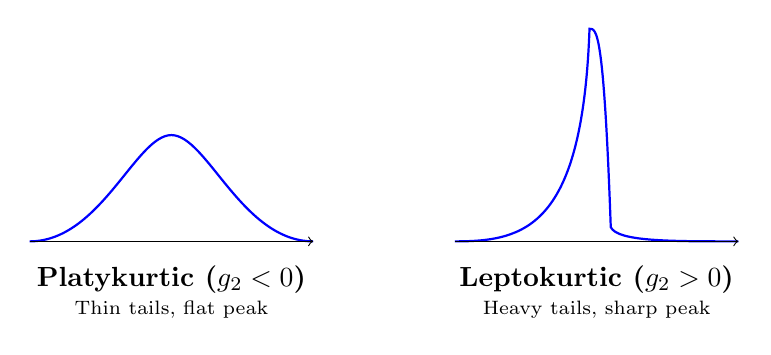
\begin{tikzpicture}[scale=0.9]
    % Platykurtic
    \begin{scope}[xshift=-4cm]
    \draw[thick, color=blue] (0,0) .. controls (1,0) and (1.5,1.5) .. (2,1.5) .. controls (2.5,1.5) and (3,0) .. (4,0);
    \draw[->] (0,0) -- (4,0);
    \node[below] at (2,-0.2) {\textbf{Platykurtic ($g_2 < 0$)}};
    \node[below, font=\scriptsize] at (2,-0.7) {Thin tails, flat peak};
    \end{scope}

    % Leptokurtic
    \begin{scope}[xshift=2cm]
    \draw[thick, color=blue] (0,0) .. controls (1,0) and (1.8,0.2) .. (1.9,3) .. controls (2,3) and (2.1,3) .. (2.2,0.2) .. controls (2.3,0) and (3,0) .. (4,0);
    \draw[->] (0,0) -- (4,0);
    \node[below] at (2,-0.2) {\textbf{Leptokurtic ($g_2 > 0$)}};
    \node[below, font=\scriptsize] at (2,-0.7) {Heavy tails, sharp peak};
    \end{scope}
\end{tikzpicture}
\end{center}

\begin{tcolorbox}[profbox, title=Imagine: The Eiffel Tower vs. Table Mountain]
\textbf{Leptokurtic (Positive Kurtosis)} looks like the Eiffel Tower: a very sharp, thin peak, but with a massive, heavy iron base sprawling outward. In data, this means heavy tails—extreme outliers are much more common than in a normal distribution (crucial to know for modeling network latency or financial risk). \\
\textbf{Platykurtic (Negative Kurtosis)} looks like Table Mountain in South Africa: a flattened top, with edges that drop off steeply like cliffs. In data, this means thin tails—outliers are exceedingly rare, and the data is tightly confined.
\end{tcolorbox}

\end{document}